\documentclass[a4paper,11pt]{article}
\usepackage[utf8]{inputenc}
\usepackage{polski}
\usepackage[polish]{babel}
\let\babellll\lll
\let\lll\relax

\usepackage{graphicx}    % Pakiet pozwalaj¹cy ,,wklejaæ'' grafikê...
\usepackage{caption}
\usepackage{subcaption}
\usepackage{epstopdf}
\usepackage{amsmath,amssymb,amsfonts,amsthm,mathtools}
                               % Do³¹czamy zestaw ró¿nych przydatnych znaczków ...
\usepackage{tikz}
\usetikzlibrary{chains,fit,shapes}

\usepackage{url}

%\usepackage{comment}  
%\usepackage[left = 2.5cm]{geometry}
%\usepackage{bbm}               % \mathbbm{N} - zbior liczb naturalnych
%tikz

\date{Wrocław, \today}
\title{\LARGE{\textbf{Rozwiązania niektórych z około dwustu łatwych zadań z języków formalnych i złożoności obliczeniowej 
(i jednego nie aż tak trudnego, jak się o nim mówi)}\\\Large{Numeracja zadań jak w zbiorze z 2017 roku}}}

\author{}

\newtheorem{innercustomthm}{Zadanie}
\newenvironment{zadanie}[1]
  {\renewcommand\theinnercustomthm{#1}\innercustomthm}
  {\endinnercustomthm}
  
\newtheorem{innercustomobs}{Obserwacja}
\newenvironment{obserwacja}[1]
  {\renewcommand\theinnercustomobs{#1}\innercustomobs}
  {\endinnercustomobs}
 

\begin{document}

\maketitle

\section{Robocze}


\section{Wskazówki}

Patrząc perspektywicznie w stronę zbliżających się egzaminów, ta sekcja wydaje mi się ważniejsza i zachęcam do spędzania z nią
czasu podczas samodzielnych wieczornych rozmyślań.

\subsection{Języki i automaty}

\begin{zadanie}{63}
Warto zastanowić się, jak miałby wyglądać niedeterministyczny automat ze stosem rozpoznający taki język. Pomocny może się też
okazać pewien lemat.
\end{zadanie}

\subsubsection{Języki rodzynkowe}

\begin{zadanie}{71}
Probem sprowadza się do rozpoznawania liter języka $L^*$. \\
Gdyby miał istanieć taki język L, to pewnie musiałby być nieskończony (dlaczego?). Może istnieje jakaś prosta, nieskończona
rodzina słów postaci $a^*ba^*$, którą automat ze stosem może łatwo rozpoznawać, ale taki bez stosu będzie miał trudniej?
Formalnie, jak to bywa, warto używać lematów.
\end{zadanie}

\subsubsection{Konfluentność}

\begin{zadanie}{74}
1) To pytanie jest (nieprzypadkowo) podobne (ale nie identyczne) do pytania: Czy każdy automat deterministyczny można 
zsynchronizować? (zadania 37-39). \\
2) Warto zauważyć, że w definicji konfluantności jest równoważność. Może zatem być tak, że obie jej strony będą zawsze fałszywe,
co oznacza, że chcemy ``na dobre'' zepsuć słowo. Może są języki nieregularne, które łatwo zepsuć?
\end{zadanie}

\begin{zadanie}{75}
To zadanie jest podobne do zadania 38.
\end{zadanie}

\begin{zadanie}{76}
Może chodzić o język, który nie jest tak łatwo zepsuć (ma długie słowa psujące).
\end{zadanie}

\subsection{Obliczalność}

\begin{zadanie}{92}
Jak coś ma nie być r.e. to na pewno chodzi o redukcję z $\overline{\mathbb{K}}$. Delikatna modyfikacja 89.
\end{zadanie}

\begin{zadanie}{99}
i) Jak coś ma nie być r.e. to na pewno chodzi o redukcję z $\overline{\mathbb{K}}$. Delikatna modyfikacja 89. \\
ii) Czy $\Phi_m \neq \Phi_n \Longleftrightarrow \exists k \Phi_m(k) \neq \Phi_n(k)$?
\end{zadanie}

\begin{zadanie}{100}
To zadanie jest podobne do zadania 102. Zaś z zadania 82 wiemy, czym jest $\Sigma_1$.
\end{zadanie}

\begin{zadanie}{101}
Trzeba wprost zdefiniować redukcję z B do A. 
\end{zadanie}

\begin{zadanie}{102}
a. założenie o nietrywialności zadania b. implikuje odpowiedź w zadaniu a.. Pewna użyteczna redukcja i w tym zadaniu okaże się
pomocna. \\
b. formalne sformułowanie tego, co to znaczy że $n \in B$, używająca 3 zmiennych, wprost prowadzi do co-r.e. zbioru A.
\end{zadanie}

\begin{zadanie}{103}
Należałoby się zastanowić, co wspólnego mają te warunki z monotonicznością f.
\end{zadanie}

\begin{zadanie}{104}
Wskazówka do implikacji $2 \Rightarrow 1$ podana w treści jest bardzo dobra. Wskazówka do implikacji odwrotnej: to jest podobne
do zadania 97. Trzeba powtórzyć tamto rozumowania, z tym że zamiast 2 zbiorów wziąć przeliczalnie wiele.
\end{zadanie}

\begin{zadanie}{110}
To jest wgl. ważne zadanie i warto mu poświęcić dłuższą chwilę. \\
a) Chcemy zakodować Maszynę Turinga (z ustalonym wejściem) jako automat deterministyczny z dwoma stosami. \\
$a_0$) Zamienić MT z ustalonym wejściem na równoważną MT z pustym wejściem. \\
$a_1$) Trzeba się przyjrzeć dokładniej temu,
jak Maszyna wygląda, porysować coś. W szczególności spostrzec, że działa ona bardzo lokalnie. Trochę podobne do zadania 
130, może być ono pewną inspiracją. \\
b) Zamienić stos na licznik. \\
$b_0$) Jak zamienić potencjalnie szeroki wybór sweterków (jak u blondynki) na sweterki tylko dwóch kolorów (jak u blondyna)? \\
$b_1$) Popatrzeć na taki zamieniony stos i zobaczyć, że w rzeczywistości wystarczy nam pamiętać jedną liczbę zamiast jednego 
stosu. \\
$b_2$) Poświęcić chwilę (!) na względnie dopracowanie wymaganych od stosów operacji w licznikowej implementacji stosów. 
Przydatne mogą okazać się dwa dodatkowe liczniki. \\
c) Zachwycić się bogactwem liczb naturalnych - w szczególności można skorzystać ze znanego wszem i wobec kodowania
skończonych ciągów liczbowych jako pojedyncze liczby. Np. ciągi 4-elementowe też się da. Zaimplementować wymagane
operacje przy użyciu drugiego licznika.
\end{zadanie}

\begin{zadanie}{114}
Mocno podobne do zadania 127 (gramatyk ze znikaniem). Tym razem trzeba zrobić dwie gramatyki, osobną dla słów $l_i$ i $r_i$.
\end{zadanie}

\begin{zadanie}{115}
Warto skorzystać z zadania 114. Udowodnić, że $(L_G)^c$ dla CFG $G$ z zad. 114 jest CFL. Porachować, przypomnieć sobie prawa
de Morgana.
\end{zadanie}

\begin{zadanie}{116}
Warto skorzystać z zadania 115.
\end{zadanie}

\begin{zadanie}{118}
Czy da się, być może dodając specyficzne zamiany, zasymulować pełny semiproces Thuego, ograniczajc się w \textbf{istotnych} 
zamianych tylko do zamiany początku pierwszego słowa na koniec drugiego?
\end{zadanie}

\section{Szkice rozwiązań}

\subsection{Języki i automaty}

\subsubsection{Synchronizacja automatów częściowych}

\begin{zadanie}{40}
\end{zadanie}

Odp: NIE. \\


\begin{figure}[h!]
  \centerline{%
    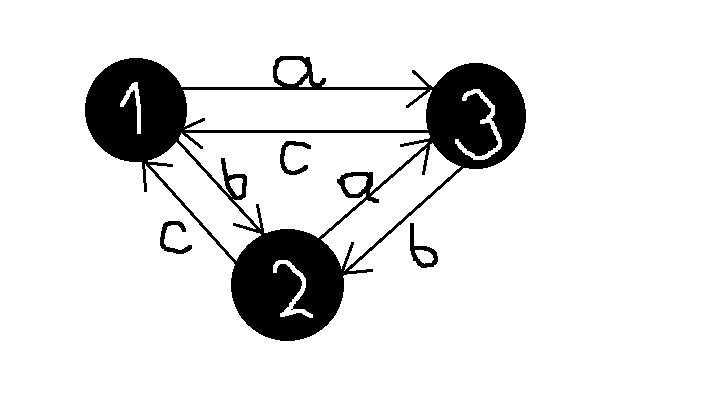
\includegraphics[width=6cm]{zad40.png}%
  }%
  \caption{$csync(\{1,2\}) \supset \{a\}; \ csync(\{1,3\}) \supset \{b\};\ csync(\{1,2\}) \supset \{c\}$. Natomiast $csync(Q) = \emptyset $.}
\end{figure}


\begin{zadanie}{41}
\end{zadanie}
W obydwu podpunktach wystarczy zbadać funkcję

\begin{align*}
 F :\ &2^Q \times \Sigma \longrightarrow 2^Q \\
 F(S,a) &= \{ \delta(q,a) : \ q \in S \}.
\end{align*}

Oczywiście $s \in csync(S) \Longleftrightarrow |\widehat{F}(S,s)| = 1$, gdy zdefiniujemy $\widehat{F}$ w naturalny sposób. 
Ponadto $1 \leqslant |F(A,a)| \leqslant |A|$, zatem $1 \leqslant |\widehat{F}(S,p)| \leqslant |S|$ dla dowolnego prefiksu $p$ słowa $s$,
czyli $\widehat{F}(S,p)$ może przyjmować co najwyżej $\displaystyle{\sum\limits^{|S|}_{k=1}\binom{|Q|}{k}}$ różnych wartości.
Oznaczmy tę liczbę jako $M$. \\ \\

Dla $|s| > M$ istnieją prefiksy $p_1$ i $p_2$ słowa $s = p_1s_1 = p_2s_2, \ |p_1| < |p_2|,$ takie że 
$\widehat{F}(S,s_1) = \widehat{F}(S,s_2)$ (Zasada Szufladkowa). Wtedy oczywiście $\widehat{F}(S,s) = \widehat{F}(S,p_1s_2)$, przy czym 
$|p_1s_2| < |s|$. \\ \\
W zwiazku z powyższym $csync(Q) \neq \emptyset \Longleftrightarrow \exists s \in S |s| \leqslant M$. \\
Dokładne odpowiedzi wynikają z tego wprost, po podstawieniu za $S$ a) dowolniego trzyelementowego zbioru stanów b) Q. \\ \\

\begin{zadanie}{42}
\end{zadanie}
Podpunkt M można rozwiązać w naturalny sposób. W kolejnych podpunktach warto jednak skorzystać ze wskazówki. \\ \\

Zbudujmy automat (częściowy) z trzech cykli, ułożonych jeden nad drugim, każdy długości m. Trzy stany, ułożene jeden nad
drugim, będą stanowiły nasz początkowy zbiór S \\ \\

\begin{figure}[h!]
  \centerline{%
    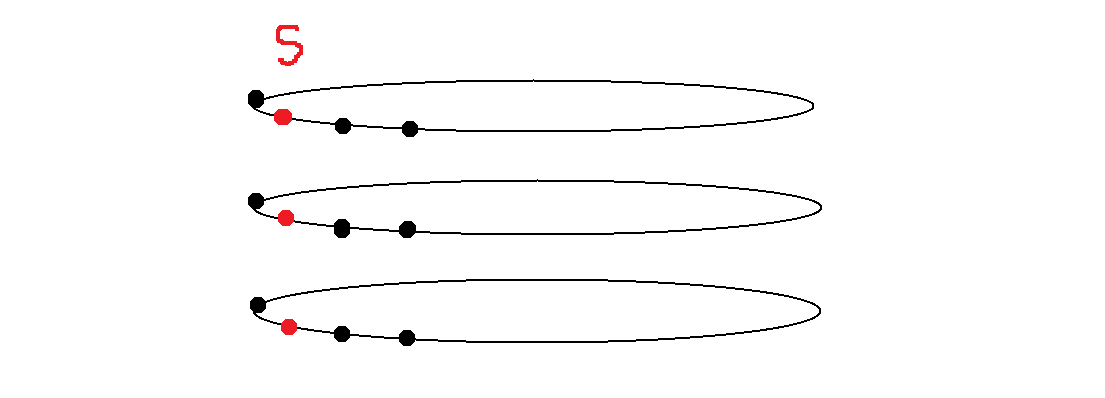
\includegraphics[width=18cm]{zad42.png}%
  }%
\end{figure}

Naszym celem jest, aby co jedną literę zmieniał się stan na górnym cyklu, co $m$ liter stan na drugim, a co $m^2$ na trzecim.
Zapenimy też, że synchronizacja będzie mogła nastąpić dopiero po przejściu przez dolny stan całego cyklu (czyli $~m^3$ krokach). \\
Możemy to wymusić w następujący sposób: \\

\begin{figure}[h!]
  \centerline{%
    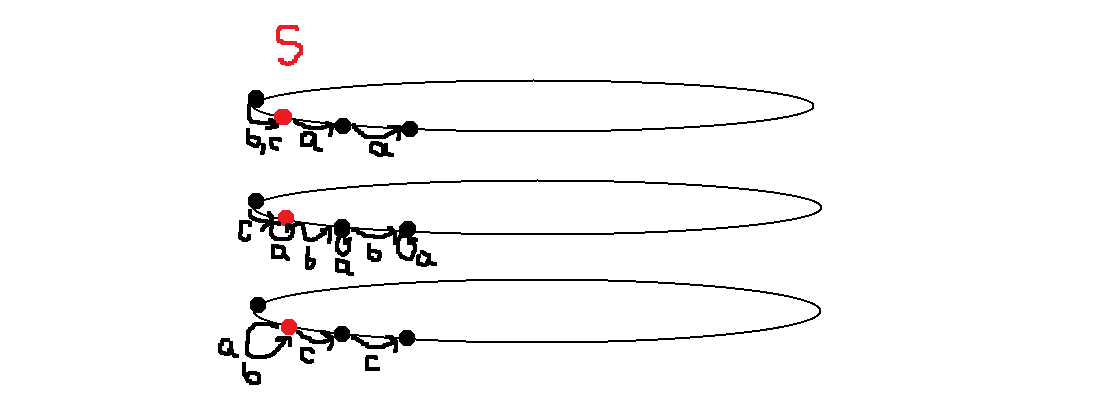
\includegraphics[width=18cm]{zad42_2.png}%
  }%
\end{figure}

przy czym pętelki z literą a są przy każdym stanie na drugim dysku, a pętelki z literami a,b są przy każdym stanie na trzecim
dysku. \\
Możliwość synchronizacji zapeniamy przez dodanie przejść z przedostatnich stanów na każdym dysku do pierwszego stanu 
dolnego dysku. Oznaczenie ich specjalną ``literką synchronizacji'', jak d, zapewni nam, że skorzystać z niej będzie można
dopiero gdy dolny stan dojdzie do przedostatniego miejsca na dolnym dysku (co następuje dopiero po $~m^3$ krokach: \\
\begin{figure}[h!]
  \centerline{%
    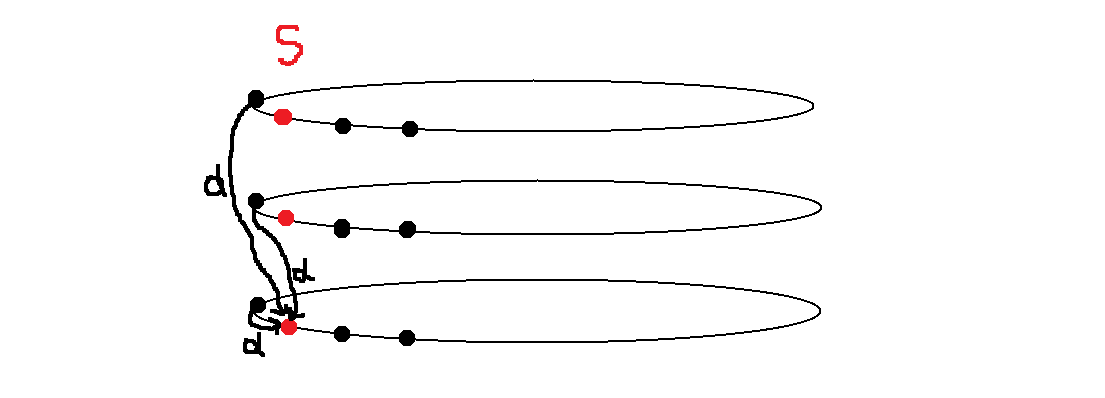
\includegraphics[width=18cm]{zad42_3.png}%
  }%
\end{figure}

Zauważmy teraz, że ten automat (zanim dojedzie do synchronizacji) jednoznacznie wyznacza słowo, dla którego funkcja przejścia 
jest określona dla wszystkich stanów z $S$:
$$
s = ((a^{m-1}b)^{m-1}c)^{m-1}d
$$
Takie $s$ synchronizuje $S$ i nie istnieje żadne krótsze od niego. Nietrudno wyliczyć, że jest ono odpowiednio długie. \\ \\



\begin{zadanie}{63}
\end{zadanie}
Przypuśćmy nie wprost, że ten język jest bezkontekstowy. Niech $N$ będzie stałą z lematu o pompowaniu dla tego języka. 
Wystarczy rozważyć słowo $0^{2N}1^{2N}0^{2N}1^{2N}$ i pamiętać, że przy podziale z lematu (ozn. $vwxyz$) zachodzi
$|wxy| \leqslant N$. Odpowiednio cierpliwe rozpatrywanie przypadków (gdzie w oryginalnym słowie ląduje podsłowo $wxy$)
prowadzi nas do wniosku, że zawsze można odpowiedni fragment podpompować (lub spompować) i uzyskać słowo spoza języka.


\subsubsection{Języki rodzynkowe}

\begin{zadanie}{71}
\end{zadanie}
Rozważmy $L = \{ a^nba^n : n \in \mathbb{N}\}$. Łatwo sprawdzić, że nawet deterministyczny automat ze stosem daje sobie radę
z językiem $L^*$, bo rozpoznawanie liter tego języka (czyli słów języka $L$) jest bardzo łatwe. \\
Z lematu o pompowaniu bardzo łatwo pokazać, że $L^*$ nie jest regularny ($L$ też nie jest).


\subsubsection{Konfluentność}

\begin{zadanie}{74}
\end{zadanie}
1) $\{ 0^n : k|n \}$ dla $k>1$ jest przykładem na regularny język niekonfluentny. \\
2) $\{ 0^n1^n : n \in \mathbb{N} \}$ jest przykładem na nieregularny język konfluentny. Uniwersalnym słowem $x$ dla tego języka
jest $10$.

\begin{zadanie}{75}
\end{zadanie}
Rozwiązanie tego zadania jest identyczne do rozwiązania zadania 38.

\begin{zadanie}{76}
\end{zadanie}
Język dobrych nawiasowań jest dobrym przykładem. Dowód przebiega nie wprost, a jeśli oznaczymy przez $c$ stałą wynikającą
z założenia nie wprost, to słowa $s_1 = \ )^{c+1}$ i $s_2 = \ (^{c+1}$ są kontrprzykładami, gdyż trzeba zepsuć $s_1$ aby je
ukonfluentnić, a nie można tego zrobić słowem długości mniejszej niż $c+2$.

\subsubsection{Transducery}

\begin{zadanie}{77}
\end{zadanie}
Podpunkt 1: definiujemy $\sigma_{Mealy} = \sigma_{Moore} \circ \delta$. Reszta zostaje.\\
Podpunkt 2: definiujemy (dla transducera Mealy'ego $\langle \Sigma, \Sigma_1, Q, q_0, \delta, \sigma_{Mealy} \rangle$)
\begin{enumerate}
 \item $Q' = Q \times \Sigma \cup q_0'$. Stan $(q,a)$ = stan do którego doszlibyśmy w starym automacie ze stanu $q$ wczytując
 literę $a$. Stan $q_0'$ - dodatkowy stan początkowy.
 \item 
 \subitem $\delta'((q,a),b) = (\delta(q,a),b)$ dla pary $(q,a) \in Q \times \Sigma$
 \subitem $\delta'(q_0',a) = (q_0,a)$
 \item
 \subitem $\sigma_{Moore}((q,a)) = \sigma_{Mealy}(q,a)$
 \subitem $\sigma_{Moore}(q_0') = \varepsilon$
\end{enumerate}
Otrzymujemy transducer Moore'a $\langle \Sigma, \Sigma_1, Q', q_0', \delta', \sigma_{Moore} \rangle$ równoważny z pierwotnym
t. Mealy'ego. \\
Dowód w obu przypadkach zapewne angażuje Zasadę Indukcji Matematycznej względem długości słowa. \\ \\ 

\begin{zadanie}{78}
\end{zadanie}
bso. (77) zajmijmy się transducerem Mealy'ego $\langle \Sigma, \Sigma_1, Q, q_0, \delta, \sigma_{Mealy} \rangle$, który 
świadczy że $A \leqslant_{reg}B$. Niech przy okazji $A_B = \langle \Sigma_1, Q^B, q_0^B, F^B, \delta^B\rangle$ będzie DFA
rozpoznającym $B$. Definiujemy $\delta'(q,a) = \widehat{\delta^B}(q,\sigma_{Mealy}(q,a))$. Udajemy, że jesteśmy słowem z języka
$B$ i chodzimy po automacie $A_B$.\\
Wtedy $\langle \Sigma, Q^B, q_0^B, F^B, \delta' \rangle$ jest DFA rozpoznającym $A$ (d-d. indukcyjny względem długości słowa). \\ \\

\begin{zadanie}{79}
\end{zadanie}
Definiujemy transducer Mealy'ego $T_{Mealy}$:
\begin{enumerate}
 \item $\Sigma = \{1,2,3,...,n\}$
 \item $Q = \Sigma$
 \item $q_0 = 1$
 \item $\delta(q,a) = a$
 \item $\Sigma_1 = Q \times \Sigma$
 \item $\sigma_{Mealy} = Id$
\end{enumerate}

Niech $T_{Moore} = \langle \Sigma, \Sigma_1, Q', q_0', \delta', \sigma_{Moore} \rangle$ będzie transducerem Moore'a 
równoważnym z $T_{Mealy}$.

\begin{obserwacja}{1}
 Możemy założyć, że każdy stan z $Q'$ jest osiągany przez DFA stowarzyszony z $T_{Moore}$. W przeciwnym razie możemy usunąć te 
 stany, a powstały $T_{Moore}'$ wciąż będzie równoważny z $T_{Mealy}$.
\end{obserwacja}

\begin{obserwacja}{2}
 $s \in Im(\sigma_{Mealy}) \Rightarrow |s| = 1$. Zatem $s \in Im(\sigma_{Moore}) \Rightarrow |s| = 1$.
\end{obserwacja}

Gdyby było $|Q'| < n^2$, to $Im(\sigma_{Mealy}) \nsubseteq Im(\sigma_{Moore})$. Niech 
$s \in Im(\sigma_{Mealy}) \setminus Im(\sigma_{Moore})$. $s = (k,l)$ dla pewnych $k,l \in \Sigma$. Rozważmy słowo
$t = kl$. Wtedy $f_{T_{Mealy}}(t) = \sigma_{Mealy}(1,k) \sigma_{Mealy}(k,l) = (1,k)(k,l)$. \\
Załóżmy nie wprost, że $f_{T_{Moore}}(t) = f_{T_{Mealy}}(t)$. Jest to równoważne (obs. 2) z tym, że 
$\sigma_{Moore}(\delta'(q_0',k)) = \sigma_{Mealy}(1,k)$ oraz 
$\sigma_{Moore}(\widehat{\delta'}(q_0',kl)) = \sigma_{Mealy}(k,l) = (k,l)$. 
Druga równość stoi w jawnej sprzeczności z naszym założeniem, że $(k,l) \notin Im(\sigma_{Moore})$.

\begin{zadanie}{80}
\end{zadanie}
Zdaje się, że świadczy o tym następujący transducer Mealy'ego:
\begin{enumerate}
 \item $\Sigma = \{(,),[,],\langle,\rangle \}$
 \item $Q = \{q_0\}$
 \item $q_0 = q_0$
 \item $\delta \equiv q_0$
 \item $\Sigma_1 = \{(,),[,] \}$
 \item
 \subitem $\sigma_{Mealy}( q_0, (/) ) = ((/)) $
 \subitem $\sigma_{Mealy}( q_0, [/] ) = [[/]] $
 \subitem $\sigma_{Mealy}( q_0, \langle / \rangle ) = [(/)] $
\end{enumerate}
Dowód pozostawiamy Czytelnikowi jako ćwiczenie. 

\subsection{Obliczalność}

\begin{zadanie}{89}
\end{zadanie}
Niech $B = \{ n : Dom(\Phi_n) = \mathbb{N} \}$. Robimy redukcję $f_{89}$ z $\overline{\mathbb{K}}$. \\
Definiujemy $f_{89}(n)$ jako numer następującego programu: \\
\texttt{wczytaj k  \\ odpal $\Phi_n(n)$ na $k$ kroków \\ jeżeli się skończył : zapętl się \\ w p.p. : zwróć 1 \\}
Sprawdzenie, że zachodzi $n \in \overline{\mathbb{K}} \Longleftrightarrow f_{89}(n) \in B$ pozostawiamy jako proste ćwiczenie.



\begin{zadanie}{92}
\end{zadanie}
Robimy redukcję $f$ z $\overline{\mathbb{K}}$. \\
Definiujemy $f(n)$ jako numer następującego programu: \\
\texttt{wczytaj k \\ jeżeli k jest parzyste : zapętl się  \\ w p.p. : \\ odpal $\Phi_n(n)$ na $k$ kroków \\ jeżeli się skończył : zapętl się \\ w p.p. : zwróć 1 \\}
Oczywiście $Dom(\Phi_{f(n)}) = (2\mathbb{N}+\{1\}) \cap \{ t \in \mathbb{N} : t < \text{czas wykonania się } \Phi_n(n) \}$. \\
Sprawdzenie, że zachodzi $n \in \overline{\mathbb{K}} \Longleftrightarrow f(n) \in B$ pozostawiamy jako proste ćwiczenie.

\begin{zadanie}{99}
\end{zadanie}
i) Robimy redukcję f z $\overline{\mathbb{K}}$, pamiętając o redukcji $f_{89}$. \\
Niech $c$ będzie numerem następującego programu: \\
\texttt{wczytaj k  \\ zwróć 1 \\}
Definiujemy $f(n) = \langle c , f_{89}(n) \rangle$. Jest oczywiste (po zrobieniu zadania $89$), że zachodzi \\
$$
n \in \overline{\mathbb{K}} \Longleftrightarrow f(n) \in T.
$$
ii) Nie. Robimy redukcję f z $\overline{\mathbb{K}}$. \\
Niech $f_a(n)$ będzie numerem następującego programu: \\
\texttt{wczytaj k \\ jeżeli k > 1 : zapętl się  \\ w p.p. : \\ odpal $\Phi_n(n)$ \\ zwróć 1 \\}
Niech $f_b(n)$ będzie numerem następującego programu: \\
\texttt{wczytaj k \\ jeżeli k > 1 : zapętl się  \\ w p.p. : \\ zwróć 1 \\}
Definiujemy $f(n) = \langle f_a(n) , f_b(n) \rangle$. Oczywiste zachodzi \\
$$
n \in \overline{\mathbb{K}} \Longleftrightarrow f(n) \in \overline{T}.
$$


\begin{zadanie}{100}
\end{zadanie}
Oczywiście $\Pi_0 = \Sigma_0$. Z zadań 81-82 wynika, że $\Sigma_1 = $ zbiory rekurencyjnie przeliczalne. Pokażemy, że
$ L \notin \Sigma_1$. Świadczy o tym następująca redukcja $f$ z $\overline{\mathbb{K}}$: definiujemy $f(n)$ jako numer
programu: \\
\texttt{wczytaj k \\ jeżeli k < n : zwróc 1 \\ w p.p. odpal $\Phi_n(n)$ \\ zwróc 1 \\}
Widzimy, że gdy $n \in \overline{\mathbb{K}}$ to  $Dom(\Phi_{f(n)}) = \{1,2,...,n\}$, w przeciwnym razie 
$Dom(\Phi_{f(n)}) = \mathbb{N}$. \\
Następnie pokażemy, że $L \in \Sigma_2$. W tym celu zdefiniujmy zbiory
\begin{align}
 B_0 = \{ \ (n,m) : &\left( \exists l<\pi_1(f^{-1}(m)) \ \Phi_n(l) \text{ zakończy się po $ \pi_2(f^{-1}(m)) $ krokach} \right) \wedge \notag \\ 
 &\left( \forall l \geqslant \pi_1(f^{-1}(m)) \ \Phi_n(l) \text{ nie kończy się} \right) \ \} \notag \\
 B = f(B_0) \notag
\end{align}
gdzie $f$ jest naszą ustaloną, obliczalną bijekcją $\mathbb{N}^2 \longrightarrow \mathbb{N}$, natomiast $\pi_i$ jest rzutem
na $i$-tą współrzędną. \\
Oczywiście $L$ jest rzutem zbioru $B_0$, zatem żeby uzasadnić, że $L \in \Sigma_2$, wystarczy pokazać, 
że jest on $B \in \Pi_1$. Dowód tego faktu pozostawiamy jako ćwiczenie.


\begin{zadanie}{101}
\end{zadanie}
Definiujemy $f^{-1}$ w następujący sposób: \\
\texttt{wczytaj n \\ Dla $k=1,2,3...$ : \\ jeżeli $f(k) = n$ : zwróć k \\ }
Oczywiście $f^{-1}$ jest całkowita, bo $f$ jest ``na". Łatwo sprawdzić, że zachodzi również $f \circ f^{-1} = Id$ 
(a czy $f^{-1} \circ f = Id$?). \\
Pokażemy, że $f^{-1}$ jest redukcją z $B$ do $A$ :
\begin{align}
 n \in B \Longleftrightarrow Id(n) \in B \Longleftrightarrow f(f^{-1}(n)) \in B \Longleftrightarrow f^{-1}(n) \in A, \notag 
\end{align}
przy czym ostatnia równoważność wynika z tego, że $f$ jest redukcją z $A$ do $B$. Oczywiście powyższe oznacza doładnie to,
że $f^{-1}$ jest redukcją z $B$ do $A$.



\begin{zadanie}{102}
\end{zadanie}
a) Nie. Wysztarczy pokazać redukcję z $\mathbb{K}$ (dlaczego?). O dziwo, jest to dokładnie $f_{89}$. \\

b) Definiujemy $A = \{ (n,k,t) : \Phi_n(i) \text{ kończy się po co najwyżej $t$ krokach dla } \\ 
i=1,2,...,k \text{ oraz nie kończy się dla $i > k$} \}$. Ten zbiór jest dobry, a sprawdzenie pozostawiamy jako ćwiczenie.


\begin{zadanie}{103}
\end{zadanie}
a) Tak. Bo istanieje takie duże $N$, że na zbiorze $\{ N, N+1, ... \}$ $f$ jest niemalejąca. Z zadania $86$ wynika więc, 
że $f(\{ N, N+1, ... \})$ jest rekurencyjny. Zatem $f(\mathbb{N}) = f(\{ 1,2, ... ,N-1 \}) \cup f(\{ N, N+1, ... \})$ jest
rekurencyjny, jako suma dwóch zbiorów rekurencyjnych. \\

b) Nie. Niech $A = \{1\}$. Niech $g$ będzie całkowitą funkcją rekurencyją, taką że $g(\mathbb{N}) = \mathbb{K}$ 
(skądinąd wiemy, że taka istnieje - np. $87$). Rozważmy następującą funkcję $f$: \\
\texttt{wczytaj n \\ jeżeli n jest parzyste : zwróć $g(\frac{n}{2})$ \\ w p.p. : zwróć 1 \\}
$f$ spełnia warunek z zadania, ale $f(\mathbb{N}) = \mathbb{K} \cup \{ 1 \}$, a to nie jest zbiór rekurencyjny.

\begin{zadanie}{104}
\end{zadanie}
$1 \Rightarrow 2$: \\
Niech $\mathbb{D} = \{ A_i : i \in \mathbb{N} \}$. Niech $\phi: \mathbb{N}^2 \longrightarrow \mathbb{N}$ będzie dowolną ustaloną
obliczalną bijekcją. Definiujemy zbiór $B$ następująco: \\
\begin{align}
 \varphi(i,n) \in B \Longleftrightarrow n \in A_i \notag
\end{align}
Ten zbiór jest dobry, a o tym, że $A_i \leqslant_{rek} B$, świadczy redukcja $\varphi(i,\cdot)$. \\
$2 \Rightarrow 1$: \\
Odpowiedź na pytanie ze wskazówki: 1. Jest to zbiór $f^{-1}(B)$. Z tego wynika, przy uwzględnieniu faktu, że redukcji 
(jako programów), jest tylko przeliczalnie wiele, że dla ustalonego zbioru $B$ istanieje tylko przeliczalnie wiele zbiorów
$A_i$ takich, że $A_i \leqslant_{rek} B$. Zatem, z tego, że $\mathbb{D} \subseteq \{ A_i : i \in \mathbb{N} \}$ wynika, że
zbiór $\mathbb{D}$ musi być przeliczalny.

\begin{zadanie}{105}
\end{zadanie}
Uwaga: $N_{emp}$ jest r.e. Semi-rozstrzyga go następujący program $\Phi_{N_{emp}}$: \\
\texttt{wczytaj n \\ dla $k=1,2,3,...$ : \\ odpal $\Phi_n(i)$ na $k$ kroków dla $i=1,2,...,k$ \\ jeżeli na którymś z argumentów $\Phi_n$ się zatrzymał : zwróć 1 \\}

a) Tak. Świadczy o tym następująca redukcja $f$: \\
Jako $f(n)$ przyjmijmy numer następującego programu: \\
\texttt{wczytaj k \\ odpal $\Phi_{N_{emp}}(n)$ \\ zwróć 1 \\}
Dowód poprawności pozostawiamy jako ćwiczenie. \\

b) Nie, bo $Tot$ nie jest r.e. (zadanie $89$), a $N_{emp}$ jest.\\


\begin{zadanie}{110}
\end{zadanie}
Bso. przyjmujemy, że mamy Maszynę Turinga z pustą taśmą wejściową i alfabetem złożonym z 0 i 1 oraz symbolu pustej taśmy - B. \\
a) Bedziemy utrzymawać jako stan automatu ze stosami dwie części aktualnie używanego skrawka taśmy MT: na lewo i na prawo od
głowicy (lewy i prawy stos). W stanie będziemy pamiętali aktualny stan MT oraz komórkę na której jest głowica 
($Q' = Q \times \Sigma$). \\

\begin{tikzpicture}
\tikzstyle{every path}=[very thick]

\edef\sizetape{0.7cm}
\tikzstyle{tmtape}=[draw,minimum size=\sizetape]
\tikzstyle{tmhead}=[arrow box,draw,minimum size=.5cm,arrow box
arrows={east:.25cm, west:0.25cm}]

%% Draw TM tape
\begin{scope}[start chain=1 going right,node distance=-0.15mm]

    \node [on chain=1,tmtape] (begin) {$\#$};
    \node [on chain=1,tmtape] {0};
    \node [on chain=1,tmtape] {1};
    \node [on chain=1,tmtape] (input) {1};
    \node [on chain=1,tmtape] {1};
    \node [on chain=1,tmtape] {0};
    \node [on chain=1,tmtape] {0};
    \node [on chain=1,tmtape] {B};
    \node [on chain=1,tmtape] {B};
    \node [on chain=1,tmtape] {B};
    \node [on chain=1,tmtape,draw=none] {$\ldots$};
\end{scope}

%% Draw TM head below (input) tape cell
\node [tmhead,yshift=-.3cm] at (input.south) (head) {$q_i$};
\end{tikzpicture}

zamieniamy na \\

\begin{tikzpicture}
 \tikzstyle{every path}=[very thick]

\edef\sizetape{0.7cm}
\tikzstyle{tmtape}=[draw,minimum size=\sizetape]
\tikzstyle{tmhead}=[arrow box,draw,minimum size=.5cm,arrow box
arrows={east:.25cm, west:0.25cm}]

%% Draw TM tape
\begin{scope}[start chain=1 going below, start chain=2 going below ,node distance=-0.15mm, every node/.style=draw]
    \node [on chain=1,tmtape,draw=none] {};
    \node [on chain=1,tmtape] {1};
    \node [on chain=1,tmtape] {0};
    \node [on chain=1,tmtape] (begin) {$\#$};
    
    \node [tmhead,right=1.15cm] at (begin.west) (head) {$(q_i,1)$};
    
    \node [on chain=2,right=3cm,tmtape] {1};
    \node [on chain=2,tmtape] {0};
    \node [on chain=2,tmtape] {0};
    \node [on chain=2,tmtape] (begin) {$\#$};
\end{scope}


\end{tikzpicture}
\\\
Operacje MT implementuje się w prosty sposób. \\
b) zamienimy stos na licznik: patrzeć na stos jako na liczbę w systemie binarnym (najbardziej
znaczące cyfry na dole stosu). Dodatkowo, aby uniknąć kłopotu z zerami wiodącymi, traktujemy symbol dna stosu $\#$ jako 1.\\
Operacje stosowe (zdejmowanie i dodawanie symboli) implementujemy jako odpowiednio 
dzielenie całkowite oraz mnożenie przez 2 + ewentualne dodanie 1 . Do tego wykorzystujemy pozostałe dwa liczniki. \\
c) konfiguracja 4 liczników jest ciągiem 4 liczb naturalnych $(a,b,c,d)$. W związku z tym w prosty sposób można ją zakodować
jako jedną liczbę równą $2^a3^b5^c7^d$. Drugi licznik jest potrzebny do implementacji wymaganych operacji na 4 licznikach:
dodawania i odejmowania ze starego licznika $\longrightarrow$ mnożenia i dzielenia nowego licznika przez odpowiednią liczbę. 
Ponadto łatwo sprawdzać, czy któryś ze starych liczników jest pusty - wystarczy sprawdzić podzielność przez odpowiednią liczbę. \\ 


\begin{zadanie}{114}
\end{zadanie}
Redukcja z PCP do problemu niepustego przekroju gramatyk: \\
Dostajemy instancję PCP: $P = \{ \langle l_i, r_i \rangle : i \in \{ 1,2,...,n \} \}$. Budujemy następujące gramatyki $G$ i $H$: \\
\begin{enumerate}
 \item $N = \Sigma \cup \{1,2,...,n\}$
 \item $T = \{ S \}$
 \item $\Pi_G = \{ S \longrightarrow l_i S i \ | \ \varepsilon \}$
 \item $\Pi_H = \{ S \longrightarrow r_i S i \ | \ \varepsilon \}$
\end{enumerate}
Oczywiście $L_G \cap L_H \neq \emptyset \, (\{ \varepsilon \}) \Longleftrightarrow $ zadana instancja PCP ma rozwiązanie.

\begin{zadanie}{115}
\end{zadanie}
Skoro języki $L_G$ i $L_H$ z zadania 114 są rozpoznawane w naturalny sposób przez deterministyczne automaty ze stosem,
to ich dopełnienia są rozpoznawane przez dopełnicze automaty $\Rightarrow$ języki $L_G^c$ i $L_H^c$ są bezkontekstowe. 
Z praw de Morgana rachunku zbiorów wynika, że
\begin{align}
 L_G \cap L_H = (L_G^c \cup L_H^c)^c \notag
\end{align}
czyli $L_G \cap L_H = \emptyset  \Longleftrightarrow (L_G^c \cup L_H^c) = A^* \Longleftrightarrow $ zadana instancja PCP 
nie ma rozwiązania. \\
Teraz wystarczy pokazać, jak program ma wygenerować gramatykę dla $L_G^c \cup L_H^c$, co będzie redukcją z dopełnienia PCP,
które jest oczywiście nierozstrzygalne. Być może najłatwiej zbudować deterministyczny automat ze stosem, rozpoznający $L_G$,
i powiedzieć, że ponieważ jest deterministyczny, to można wywrócić stany akceptujące na lewą stronę i dostaniemy automat rozpoznający
dopełnienie. A z niego można wyprodukować gramatykę (ponoć wykład).

\begin{zadanie}{116}
\end{zadanie}
Nie. Redukcja z zadania 115: \\
Weż gramatykę $G$ z problemu $L_G =? A^*$. Wyprodukuj gramatykę $G_{all}$, taką że $L_{G_{all}} = A^*$. Zwróć parę gramatyk
$G$ i $G_{all}$. \\
Oczywiście zachodzi $L_G = A^* \Longleftrightarrow L_G = L_{G_{all}}$, co kończy dowód poprawności.

\begin{zadanie}{118}
\end{zadanie}
Redukcja z semiThuego: \\
Dostajemy zbiór produkcji P oraz słowa v i w. Idea: zapętlić słowo (skleić początek z końcem), dodając przy tym specjalny
znak początku słowa ($\#$). Formalnie:
\begin{enumerate}
 \item $\Sigma' = \Sigma \cup \{ \# \}$
 \item $v' = \# v$
 \item $w' = \# w$
 \item $P' = P \cup \{ \langle a , a \rangle : a \in \Sigma' \}$
\end{enumerate}
Implikacja w prawo jest, jak zwykle, dość oczywista. Do implikacji w lewo trzeba uzasadnić przekonywująco, że jeżeli 
$v' \longrightarrow_{P'}^* w'$, to można naśladować potrzebne produkcje i z $v$ otrzymać $w$ w zwykłym semiThu. 


\end{document}
